\section{Requirement and Overview}\label{sec:pilotstudy}

As surveyed in Section~\ref{sec:relatedwork}, there are two main steps to augment the node-link diagram: information extraction and description. Thus, we conducted a pilot study aiming to investigate the requirements for these two steps from the viewpoints of both 3 experts (P1-3) and 12 end-users (P4-15). We showed them some typical and various sample node-like diagrams with legends. Based on their relevant feedback, we analyzed the approach requirement and proposed an overview of our approach.

\subsection{Requirement Analysis}

Based on our analysis, we came up with four requirements [E1-4] for information extraction and three requirements [D1-3] for description generation.

\noindent {\bf Extracting Information.}

\begin{compactenum}[\textbf{E}1]
    \item {\bf Searching link condition.} The meanings of links should be demonstrated directly to end-users. Unlike nodes, users cannot find the meaning of a link on the title or caption of a graph. Hence, all experts suggested we summarize the meanings of links for users before they carefully analyze the graph. Experts also gave more refined suggestions pertaining to our approach of finding the correct link condition~\cite{DBLP:journals/ivs/LiuNS14, DBLP:journals/ivs/HeerP14, DBLP:journals/tvcg/SrinivasanPEB18} among nodes to help users understand the meaning of links automatically.
    
    \item {\bf Summarizing visual encodings.} Visual encoding is a necessary part for users to understand the graph. Although legends always represent it, they are too concise for users to understand. Furthermore, both P4 and P7 commented that despite their ability to comprehend visual encodings, it was wasteful to search attributes for each node and link according to their visual elements and legends. Thus, it is highly recommended to summarize all visual encodings, which can be demonstrated directly to users later.
    
    \item {\bf Identifing the layout type.} All experts agreed that the layout could help users understand the node-link diagram. Whereas, due to the lack of prior knowledge, most end-users ignored the layout. Experts recommended that we present only the essential information and type of layout rather than explain the algorithm details in detail to reduce end-users' understanding load. Expert P2  suggested only identifying whether the layout is topology-driven or attribute-driven, or neither, according to the taxonomy~\cite{DBLP:journals/cgf/NobreMSL19}. 
    
    \item {\bf Utilizing multi-source inputs}. Experts suggested our approach should utilize multi-source inputs, especially the original data and the visualization program. Expert P1 emphasized the importance of visualization programs, since they contain more information, such as how data attributes are encoded by visual channels, than raw data. Enriching the types of our inputs can improve the accuracy and the comprehensiveness of the collected information to avoid misleading users.
\end{compactenum}

\noindent {\bf Describing information. }
\begin{compactenum}[\textbf{D}1]
    \item {\bf Describing information with textual descriptions.} Most end-users prefer our method as it can use more detailed hints such as textual descriptions to provide more comprehensive illustrations. 
    % They mentioned that the common used legend is troublesome, first, they need to learn the mapping relationship, second, they should interpret each visual element one by one by searching the corresponding information provided by the legend. 
    Expert P2 suggested to use textual descriptions, which are more flexible to carry different content.
    The use of textual descriptions can reduce the learning cost, as well as help users focus more on analysis rather than information searching~\cite{DBLP:journals/tochi/FerresLST13, DBLP:conf/inlg/ObeidH20, DBLP:conf/apvis/LiuXHWY20}. 
    % The end-user P4 said that ``Language is the bridge of communication, and language descriptions of visualizations can bridge me to their authors.'' 
    
    \item {\bf Using templates to generate consistent descriptions.} One expert suggested that a template-based scheme is more suitable for our description generation, because it is stable and consistent to display structured descriptions in our scenario. He also suggested highlighting non-template information in the template to facilitate users' recognition.
    % End-users also prefer using template. They deemed that in tasks, they often need to find one attributes for multiple nodes. If the attributes showed on different place of descriptions, it is difficult for them to search the information and analyze.
    
    \item {\bf Organizing descriptions according to their relationship.} Because there may be several different types of information, expert P2 suggested organizing the corresponding descriptions according to their relationships. Specifically, he said that all descriptions of visual encodings of the same data entity should be displayed together without adding any additional descriptions, such as the meanings of links. It was agreed upon by all end-users that descriptions should be arranged according to the relationship as most daily document tools did, such as ``X-mind'', ``Google Doc'', ``Typora''and so on.
    
    \item {\bf Constructing mapping between graph and descriptions.} Building a linkage between our hints and the visualization can help users quickly locate and search for the target. Some end-users mentioned that the static hints (e.g., legend) obstructed their information tracking. They suggested providing an interactive mapping tool; for example, the relevant visual elements can be highlighted while hovering on their descriptions. The interactive mapping tool can make the hints more targeted and reduce mismatches with the end-users’ mental map.
\end{compactenum}

\subsection{\ApproachName~Overview} \label{sec:overview}

\begin{figure*}[t]
    \centering
    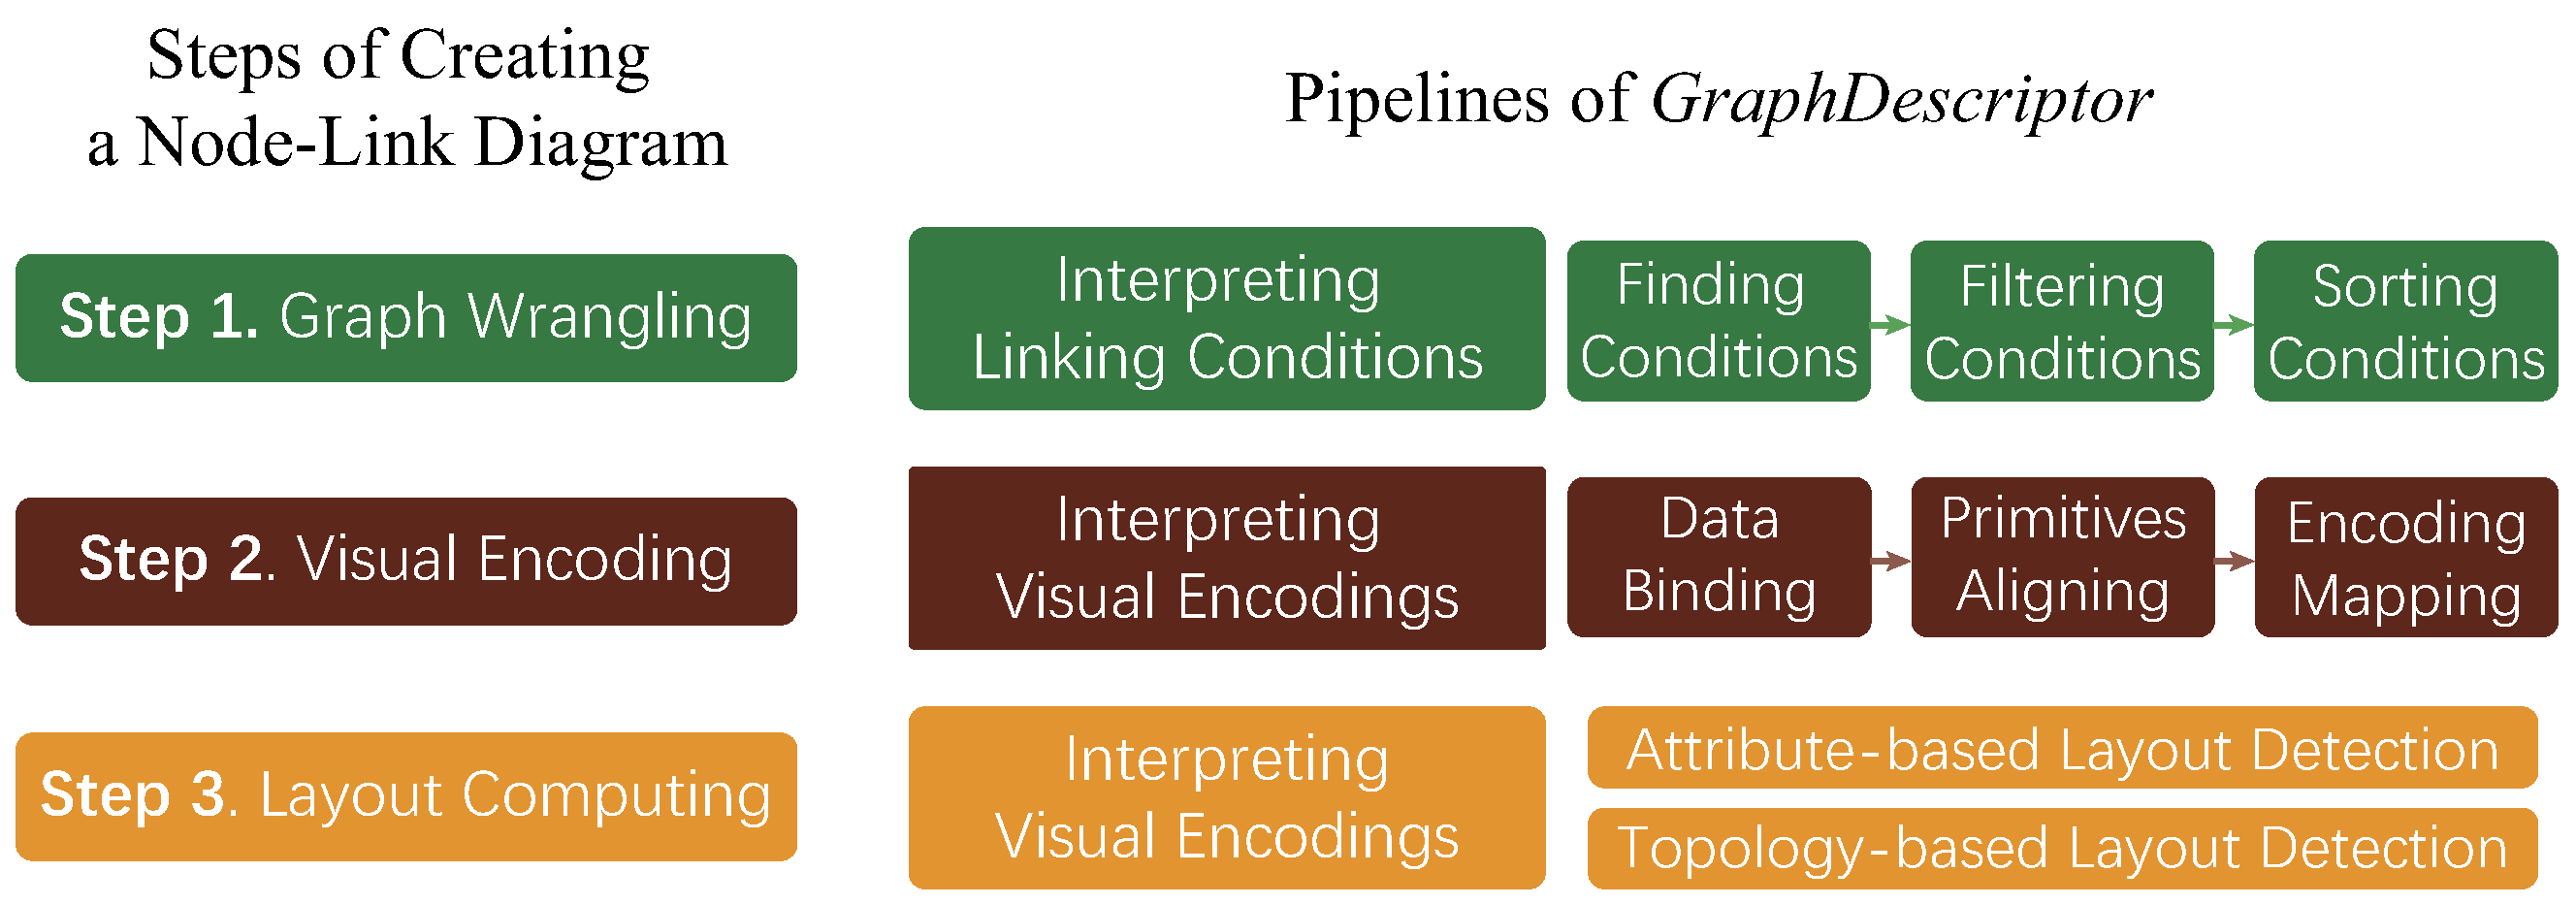
\includegraphics[width=2\columnwidth]{figures/workflow.eps}
    \caption{The pipeline of~\ApproachName. (a) Three information extraction modules search link conditions, summarize visual encodings, and identify layout types. (b) A description generator generates template-based descriptions with interactions. 
    }
    \label{fig:workflow}
\end{figure*}

Following the aforementioned requirements, we propose~\ApproachName~(Figure~\ref{fig:workflow}), an automatic description generation approach to augment the comprehensibility of node-link diagrams, which consists of three information extraction modules and an interactive description generator. They work together to extract information from node-link diagrams and generate corresponding descriptions for end-users.

\noindent {\bf Information Extraction Modules}  (Section~\ref{sec:approach}). To complete \textbf{E1-4}, we designed and implemented three information extraction modules (Figure~\ref{fig:workflow}a) with multi-source inputs (\textbf{E}) including the captured visualization programs and the original graph data.

\begin{compactenum}[\textbf{M}1]
    \item {\bf Link Condition Search Module.}
    To implement \textbf{E1}, we searched the link conditions. The module takes the original graph data as input and selects proper conditions between connected node pairs to represent the link meanings.
    
    \item {\bf Visual Encodings Summarization Module.}
    Following \textbf{E2}, our module forms the encoding scheme by summarizing mappings between data entities and visual elements and the correlations between data attributes and visual channels. It takes visualization programs and the original graph data as inputs and tests the relationship between the graph data and output visualizations to infer visual encodings.
    
    \item {\bf Layout Type Identification Module.} Based on \textbf{E3}, we proposed this module to determine whether the layout is attribute-based or topology-based. This module will capture the position of each node by computing bounding boxes, and determine the layout type by testing the Pearson correlation coefficient.
\end{compactenum}

\noindent {\bf Description Generator} (Section~\ref{sec:generator}).
According to \textbf{D1-4}, we propose a description generator
(Figure~\ref{fig:workflow}b) to express the extracted information. 
The description generation follows a manner of template-filling (\textbf{D1-2}). Although the template resembles the skeleton of the description, the spirit of the description is derived from the extracted information.
To demonstrate the relationship of different levels of descriptions (\textbf{D3}), we organized the generated descriptions in a pre-set structure. Besides, driven by \textbf{D4}, we linked them to their corresponding visual elements to reach an interactive scheme. When users hover over a description or visual element in this interactive scheme, the other element is highlighted.
